\documentclass[12pt]{article}

%TITLE
%=====
\title{\huge{\textbf{\\Two-Dimensional protodns code}}}
\author{\\ \\John C. Bowman\\University of Alberta\\Edmonton, Canada}
\date{Aug 2016}
%PAGE LAYOUT
%===========
\setlength{\oddsidemargin}{0pt}
\setlength{\evensidemargin}{0pt}
\setlength{\marginparwidth}{0pt}
\setlength{\marginparpush}{0pt}
\setlength{\marginparsep}{0pt}
\setlength{\textwidth}{464pt}
\addtolength{\topmargin}{-2.0cm}
\addtolength{\textheight}{4.0cm}

%PACKAGES
%========
\usepackage{bm}
\usepackage{amsmath}
\usepackage{mathrsfs}
\usepackage{amsfonts}
\usepackage{graphicx}
\usepackage{booktabs}
\usepackage{colordvi,color}
\usepackage{hyperref}

%MACRO DEFINITION
%================
\def\dotp{\bm{\cdot}}
\def\crossp{\bm{\times}}
\def\grad{\bm{\nabla}}
\def\div{\bm{\nabla\cdot}}
\def\curl{\bm{\nabla\times}}
\def\lap{{\nabla}^2}
\def\lapinv{{\nabla}^{-2}}
\def\so{\quad\Rightarrow\quad}
\def\soo{\qquad\Rightarrow\qquad}
\def\A{\bm{A}}
\def\S{\bm{S}}
\def\F{\bm{F}}
\def\p{\bm{p}}
\def\q{\bm{q}}
\def\r{\bm{r}}
\def\k{\bm{k}}
\def\u{\bm{u}}
\def\x{\bm{x}}
\def\OMEGA{\bm{\omega}}
\def\eI{\bm{\hat{i}}}
\def\eJ{\bm{\hat{j}}}
\def\eK{\bm{\hat{k}}}
\def\en{\bm{\hat{n}}}

%COMMANDS OPTIONS
%================
\definecolor{heavyred}{cmyk}{0,1,1,0.25}
\definecolor{heavyblue}{cmyk}{1,1,0,0.25}
\hypersetup{
  pdftitle=,
  pdfpagemode=UseOutlines,
  citebordercolor=0 0 1,
  colorlinks=true,
  allcolors=heavyred,
  breaklinks=true,
  pdfauthor=,
  pdfpagetransition=Dissolve,
  bookmarks=true
}
\hyphenation{protodns}
%BODY OF THE DOCUMENT
%====================
\begin{document}
\maketitle
\thispagestyle{empty}
\begin{figure}[h]
\centering

\includegraphics{Logo}
\end{figure}
\newpage
\thispagestyle{empty}
\begin{center}
\ \vspace{20cm}\\
John C. Bowman\\
ALL RIGHTS RESERVED\\
Reproduction of these notes in any form, in whole or in part, is permitted only for nonprofit educational use.
\end{center}
\newpage
\setcounter{page}{1}
\section{Introduction}
In this text, we are going to give a summarized yet comprehensive explanation of the \emph{protodns} code which is a \emph{Direct Numerical Simulation} code for two-dimensional incompressible homogeneous turbulent flow with priodic boundary conditions in Fourier space. Through out the context, we will explain the set of governing equations and the way through which we can obtain the most numerically efficient representation(regarding the calculation required in Fourier space) of these equations. 
Here we must mention that as it can be inferred from the name of the code, it is the simpler version of the most efficient and complete DNS code for simulation of two-dimensional incompressible homogeneous turbulent flows with periodic boundary conditions in Fourier space called \emph{2d} code. So the main reason of having \emph{protodns} is essentially for educational purposes and so it does not exploit many possible implementation optimizations to speed up the simulation process. The reader who is interested in the most advanced efficient and complete version of this code, can refer to the \emph{2d} code available at ``https://github.com/dealias/dns/tree/master/2d''.
%
\section{Governing Equations}
We start our work with the set of governing equations for incompressible turbulent flows. The main set of governing equations are Navier--Stokes equation for momentum and the incompressibilty condition:
%
%====================== Eq-1
\begin{equation}\label{Eq-1}
\begin{cases}
\dfrac{\partial \u}{\partial t} + \u\cdot\grad\u = -\grad p + \nu\lap\u + \F\\
\\
\div \u =0
\end{cases}
\end{equation}
%
There is still another possible set of equations equivalent to the equation 1 nevertheless sometimes easier to work with. That is the \emph{Vorticity} equation, and so the set of governing equations can be also represented as:
%
%====================== Eq-2
\begin{equation}\label{Eq-2}
\begin{cases}
\dfrac{\partial{\OMEGA}}{\partial t} + (\u\dotp\grad)\OMEGA=(\OMEGA\dotp\grad)\u + \nu\lap\OMEGA + \curl\F \\
\\
\div \u =0
\end{cases}
\end{equation}
%
The main advantage of using \emph{vorticity} equation instead of momentum equation is the fact that vorticity equation does not involve pressure term which in turn involves solving Poisson's equation. So as we stated above, considering our problem with periodic boundary conditions,, we do not concern about the pressure term and so the vorticity equation will save us from dealing with Poisson's equation. Taking into account that our problem is 2D, it is still possible to make use of the existence of \emph{stream} function, and so for the case of 2D incompressible turbulent flow we would have:
%
%====================== Eq-3
\begin{equation}\label{Eq-3}
\begin{cases}
\u=u(x,y)\eI+v(x,y)\eJ \\
\hspace{3.5cm}\soo \div\u=0 \\
u=-\dfrac{\partial\psi}{\partial y},\quad v=\dfrac{\partial\psi}{\partial x}
\end{cases}
\end{equation}
%
now by the definition of vorticity which is $\OMEGA=\grad\crossp\u$, then we will have:
%
%====================== Eq-4
\begin{equation}\label{Eq-4}
\OMEGA=\left(\frac{\partial v}{\partial x}-\frac{\partial u}{\partial y}\right)\eK
\end{equation}
%
which in fact shows that in the case of 2D incompressible flow, $\OMEGA$ is a vector whose direction is always prependicular to the velocity vector, so what is important is just the length of the vorticity vector. Thus, we can look at the vorticity as an scalar function. Now using the equation \eqref{Eq-3} in \eqref{Eq-4}, we will have:
%
%====================== Eq-5
\begin{equation}\label{Eq-5}
\OMEGA=(\lap\psi)\eK
\end{equation}
%
while we can write:
%
%====================== Eq-6
\begin{equation}\label{Eq-6}
\u=\frac{\partial\psi}{\partial y}\eI+\frac{\partial\psi}{\partial x}\eJ=\eK\crossp\grad\psi
\end{equation}
so using equations \eqref{Eq-5},\eqref{Eq-6}, we can represent the velocity vector with respect to the stream function as:
%
%====================== Eq-7
\begin{equation}\label{Eq-7}
\u=\eK\crossp\grad(\lapinv\omega)
\end{equation}
%
as we mentioned above, because in 2D flow, the vorticity is always prependicular to the velocity vector, and also because of incompressibility, the first term in the right hand side of the vorticity equation vanishes, so the vorticity equation will be simplified as:
%
%====================== Eq-8
\begin{equation}\label{Eq-8}
\frac{\partial{\omega}}{\partial t} + (\u\dotp\grad)\omega= \nu\lap\omega + f
\end{equation}
%
now by expanding equation\eqref{Eq-8}, we would have:
%
%====================== Eq-9
\begin{equation}\label{Eq-9}
\frac{\partial{\omega}}{\partial t} + (\eK\crossp\grad(\lapinv\omega)\dotp\grad)\omega= \nu\lap\omega + f
\end{equation}
using the inverse discrete Fourier transform, we would have:
%
%====================== Eq-10
\begin{align}%\label{Eq-10}
\omega(\x)&=\sum_{\p}{e^{i\p\dotp\x}\omega(\p)}=\sum_{\p}{e^{i\p\dotp\x}\omega_{\p}} 		  \notag 
\\
(\eK\crossp\grad(\lapinv\omega(\x))\dotp\grad)\omega(\x) &=(\eK\crossp\grad(\lapinv\sum_{\p}{e^{i\p\dotp\x}\omega_{\p}})\dotp\grad)\sum_{\q}{e^{i\q\dotp\x}\omega_{\q}} 								  \notag 
\\
&=\sum_{\p,\q}{\frac{(\eK\crossp\p)\dotp\q}{|\p|^2}\omega_{\p}\omega_{\q}e^{i(\p+\q)\dotp\x}} \notag 
\\
\nu\lap\omega(\x)&=\nu\sum_{\p}{|\p|^2e^{i\p\dotp\x}\omega_{\p}} 							  \notag 
\\
f(\x)&=\sum_{\p}{e^{i\p\dotp\x}f_{\p}} \label{Eq-10}
\end{align}
%
now, using \eqref{Eq-10} and taking discrete Fourier transform of \eqref{Eq-9}, we have:
%
%====================== Eq-11
\begin{equation}\label{Eq-11}
\frac{\partial}{\partial t}({\sum_{\p,\r}{e^{i(\p-\r)\dotp\x}\omega_{\p}}}) + \sum_{\p,\q,\r}{\frac{(\eK\crossp\p)\dotp\q}{|\p|^2}\omega_{\p}\omega_{\q}e^{i(\p+\q-\r)\dotp\x}}= \nu\sum_{\p,\r}{|\p|^2e^{i(\p-\r)\dotp\x}\omega_{\p}} + \sum_{\p,\r}{e^{(i\p-\r)\dotp\x}f_{\p}}
\end{equation}
%
so by simplifying the above equation, the final governing equation in the wave space(Fourier space) would be:
%
%====================== Eq-12
\begin{equation}\label{Eq-12}
\frac{\partial\omega_{\r}}{\partial t} + \sum_{\p}{\frac{(\eK\crossp\p)\dotp\r}{|\p|^2}\omega_{\p}\omega_{\r-\p}}= -\nu{|\r|}^2\omega_{\r} + f_{\r}
\end{equation}
%
Although the equation \eqref{Eq-12} is obtained as the governing equation in Fourier space that must get solved numerically, but that representation is not used in action. So for finding the practical governing equation, we can represent the equation \eqref{Eq-12} in the following form:
%
%====================== Eq-13
\begin{equation}\label{Eq-13}
\frac{\partial\omega_{\k}}{\partial t} + \mathcal{F}\{\u\cdot\grad\omega\}= -\nu{|\k|}^2\omega_{\k} + f_{\k}
\end{equation}
%
so as it was presented above $u,v$ can be obtained based on the $\omega$, and this is what that makes the numerical simulation easier as it is represented in the next section.
%
\section{Numerical Simulation}
\subsection{The Domain of Simulation}
Now that we have our governing equation \eqref{Eq-13} in Fourier space, then we need to take a numerical scheme to solve that equation. So at first we need to characterize our domain of simulation. As we mentioned before, because our intention is direct numerical simulation of homogeneous isotropic turbulence, so we have to avoid having walls or in fact we have to stay far enough from walls. This can be easily done by considering periodic boundary conditions. Considering this point, our schematic domain is shown in Figure (\ref{Fig-1}). 
%====================== Fig-1
\begin{figure}[h]
\centering
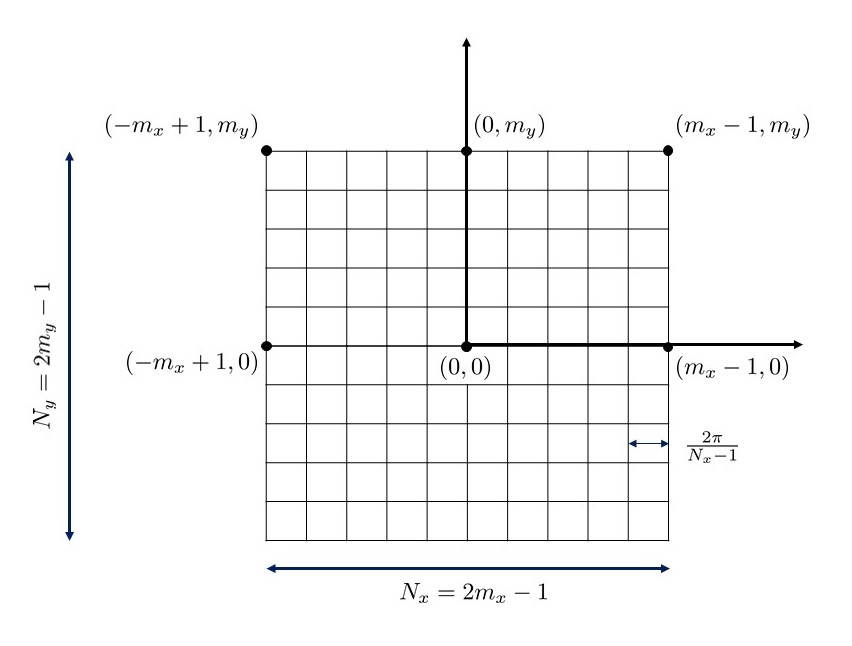
\includegraphics{domain}
\caption{Domain of simulation}\label{Fig-1}
\end{figure}
%
\subsection{Solution Algorithm}
Now, we are to represent the numerical scheme that we have to take for solving our governing equation. As we stated in the previous section, the governing equation is:
%
%====================== Eq-14
\begin{equation}\label{Eq-14}
\frac{\partial\omega_{\k}}{\partial t} + \mathcal{F}\{\u\cdot\grad\omega\}= -\nu{|\k|}^2\omega_{\k} + f_{\k}
\end{equation}
%
This equation can be written as an evolutional equation for $\omega$ by taking all the terms except the time-derivative of $\omega$ to the right-hand side:
%
%====================== Eq-15
\begin{equation}\label{Eq-15}
\frac{\partial\omega_{\k}}{\partial t} =- \mathcal{F}\left\lbrace u\dfrac{\partial \omega}{\partial x}+v\dfrac{\partial \omega}{\partial y}\right\rbrace -\nu{|\k|}^2\omega_{\k} + f_{\k} :=S_{\k}
\end{equation}
%
The numerical solution steps are as the following steps:
\begin{enumerate}
\item Initialize $\omega_{\k}$ in the Fourier space
\item Calculate velocity components $u,v$ based on $\omega$.
\item Take the inverse discrete fast Fourier transform($FFT^{-1}$) of $u,v,\omega$ to go to physical space
\item Calculate the multiplicative terms appeared in the inertial term in physical space
\item Take the discrete fast Fourier transform($\text{FFT}$) of the multiplicative terms to get back to Fourier space
\item Update the values of $\omega$ by marching one step in time
\item Calculate the values of Energy, Enstrophy, and Planenstrophy
\item Go to the step 2.
\end{enumerate}
The flowchart of the above numerical algorithm is shown in Figure (\ref{Fig-2}).
%
%====================== Fig-2
\begin{figure}[h]
\centering
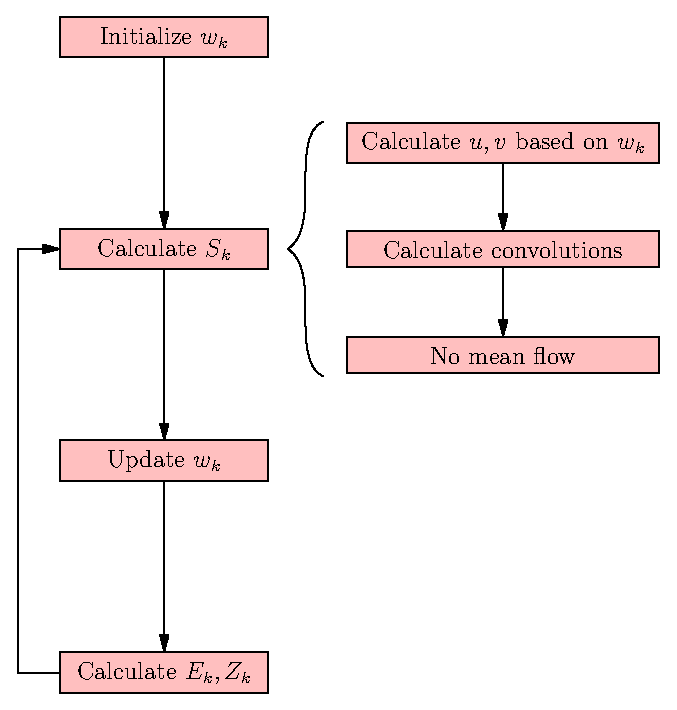
\includegraphics{algorithm}
\caption{Solution algorithm}\label{Fig-2}
\end{figure}
%
\section{Governing Equations Revisited}
Counting the number of $\text{FFTs}$ required for the numerical solution of the equation \eqref{Eq-15}, it can be observed that there are 5 $\text{FFTs}$ (three inverse $\text{FFTs}$ for $u,v,\omega$, and two forward for the multiplicative terms. Now, it is possible to ask is it generally possible to reduce the number of $\text{FFTs}$ required in the numerical solution as they are the most expensive parts of calculation(regarding CPU time)?\\
The answer is positive if we rewrite the governing equation more intelligently using some sort of symmetries available by using incompressibility. This was done both for 2D and 3D cases by C. Basdevant (1982), however it seems that it has not been well appreciated during these years. In the following, we will represent this kind of formulation of vorticity equation. At the end, the reader will notice that this approach will reduce the number of required $\text{FFTs}$ from 5 to 4. Regarding the fact that taking fast Fourier transforms(both forward or backward) is the most expensive part of the calculation, it can be easily understood that this new representation of governing equations can significantly speed up the solution. \\
we start with inertial term in vorticity equation:
%
%====================== Eq-16
\begin{equation}\label{Eq-16}
\u\cdot\grad\omega=u\dfrac{\partial \omega}{\partial x}+v\dfrac{\partial \omega}{\partial y}
\end{equation}
%
now using incompressibility, we can rewrite the inertial terms(I.T):
%
%====================== Eq-17
\begin{equation}\label{Eq-17}
\text{I.T.} :=u\dfrac{\partial \omega}{\partial x}+v\dfrac{\partial \omega}{\partial y}=\dfrac{\partial (u\omega)}{\partial x}+\dfrac{\partial (v\omega)}{\partial y}
\end{equation}
%
on the other hand:
%
%====================== Eq-18
\begin{equation}\label{Eq-18}
\omega=\left(\dfrac{\partial v}{\partial x}-\dfrac{\partial u}{\partial y}\right)
\end{equation}
%
so we can write:
%
%====================== Eq-19
\begin{equation}\label{Eq-19}
\text{I.T.} =\dfrac{\partial (u\omega)}{\partial x}+\dfrac{\partial (v\omega)}{\partial y}=\dfrac{\partial}{\partial x} \left(u\dfrac{\partial v}{\partial x}-u\dfrac{\partial u}{\partial y}\right)+\dfrac{\partial}{\partial y} \left(v\dfrac{\partial v}{\partial x}-v\dfrac{\partial u}{\partial y}\right)
\end{equation}
%
so we can write:
%
%====================== Eq-20
\begin{align}\label{Eq-20}
\text{I.T.} &= \dfrac{\partial}{\partial x} \left(u\dfrac{\partial uv}{\partial x}-v\dfrac{\partial u}{\partial x}-\dfrac{1}{2}\dfrac{\partial u^2}{\partial y}\right)+\dfrac{\partial}{\partial y} \left(\dfrac{1}{2}\dfrac{\partial v^2}{\partial x}- \dfrac{\partial uv}{\partial y}-u\dfrac{\partial v}{\partial y}\right) \notag \\
&= \dfrac{\partial^2 (uv)}{\partial x^2}-\dfrac{1}{2}\dfrac{\partial^2 u^2}{\partial x \partial y}-\dfrac{\partial }{\partial x}\left(v\dfrac{\partial u}{\partial x}\right)+\dfrac{1}{2}\dfrac{\partial^2 v^2}{\partial x \partial y}-\dfrac{\partial^2 (uv)}{\partial y^2}+\dfrac{\partial }{\partial y}\left(u\dfrac{\partial v}{\partial y}\right) \\
&= \left(\dfrac{\partial^2}{\partial x^2}-\dfrac{\partial^2}{\partial y^2}\right)(uv)+\dfrac{1}{2}\dfrac{\partial^2}{\partial x \partial y}\left(v^2 - u^2 \right)+\dfrac{\partial }{\partial y}\left(u\dfrac{\partial v}{\partial y}\right)-\dfrac{\partial }{\partial x}\left(v\dfrac{\partial u}{\partial x}\right) \notag
\end{align}
%
now, again by using incompressibility for the last two terms on the right-hand side, we will have:
%
%====================== Eq-21
\begin{equation}\label{Eq-21}
\text{I.T.} =\left(\dfrac{\partial^2}{\partial x^2}-\dfrac{\partial^2}{\partial y^2}\right)(uv)+\dfrac{\partial^2}{\partial x \partial y}\left(v^2 - u^2 \right)
\end{equation}
%
so the vorticity equation in Fourier space can be written using the above formulation:
%
%====================== Eq-22
\begin{equation}\label{Eq-22}
\frac{\partial\omega_{\k}}{\partial t} =- \mathcal{F}\left\lbrace\left(\dfrac{\partial^2}{\partial x^2}-\dfrac{\partial^2}{\partial y^2}\right)(uv)+\dfrac{\partial^2}{\partial x \partial y}\left(v^2 - u^2 \right)\right\rbrace-\nu{|\k|}^2\omega_{\k} + f_{\k} :=S_{\k}
\end{equation}
%
now it can be observed that having $u,v$ in the physical space is enough to calculate two new terms, $(uv), (v^2 - u^2)$, and consequently we will need totally 4 $\text{FFTs}$.
\end{document}





